\documentclass{bmvc2k}

\usepackage{color}
\usepackage{setspace}
\usepackage{subfigure}
\usepackage{overpic}
\usepackage[linesnumbered,ruled,vlined]{algorithm2e}
\SetKw{Continue}{continue}
\renewcommand\thesubsection{\Alph{subsection}}

\begin{document}
	
\section*{Supplementary}

\subsection{Improved IOU Tracker Algorithm}
A detailed description of our improved IOU tracker method is shown in Algorithm \ref{alg:iou-tracker}, where $D_f$ denotes the detections at frame $f$, $d_j$ the $j^{th}$ detection at the frame, $\Delta_f$ the displacements of corresponding detections in frame $f$ and $f+1$, $\delta_j$ the displacements of $j^{th}$ detection in frame $f$, $T_{\alpha}$ active tracks, $T_f$ finished tracks, $ttl$ the maximum number of virtual detections and $F$ the number of frames in the sequence. 

Fed with a set of detections and displacements, the algorithm first filters detections with a confidence threshold $\sigma_{low}$. Then for each track $t_i$ in $T_{\alpha}$, if IOU of $t_i$ and a detection in current frame is larger than threshold $\sigma_{iou}$, it will be treated as a good association and the track will be updated. Otherwise, a virtual detection will be assigned to $t_i$. If the number of virtual detections in $t_i$ is greater than $ttl$, then $t_i$ will be considered as a finished track and added to $T_f$ after filtered by track confidence and length. Virtual detections can fill the gaps caused by missing detection and thus reduce fragmentation in multi-object tracking. Compared with original algorithm, a 3D IOU is used in our approach, and each detection $d_j$ is adjusted with its displacement $\delta_j$ from previous frame. The improvement is highlight in red.

\vspace{-0.3cm}
\begin{algorithm}
	\small
	\caption{Improved IOU Tracker}
	\label{alg:iou-tracker}
	\textbf{Input: }
	$D=\{D_0,D_1,...,D_{F-1}\} = \{\{d_0, d_1, ..., d_{N_0}\},..., \{d_0, d_1, ..., d_{N_{F-1}}\}\}$,
	$\Delta=\{\Delta_0, \Delta_1, ..., \Delta_{F-1}\} = \{\{\delta_0, \delta_1, ..., \delta_{N_0}\},...,\{\delta_0, \delta_1, ..., \delta_{N_{F-1}}\}\}$\\
	\textbf{Output: } $T_f$\\
	\textbf{Initialize:} $T_a=\phi,T_f=\phi, D = \{\{D_i \mid d_i \in D_j, d_j \leq \sigma_{low}\} \mid D_j \in D\}$
	
	\For{$f=0$ to $F$}
	{
		\For{$t_i\in T_a$}
		{
			$d_{best} = d_j$ where $max(\textcolor[rgb]{1,0,0}{IOU_{3d}(d_j+\delta_j, t_i)}), d_j \in D_f, \delta_j \in \Delta_f$\\
			\If{$IOU_{3d}(d_{best},t_i)\geq \sigma_{iou}$}
			{
				replace virtual detections in $t_i$ through interpolation\\
				add $d_{best}$ to $t_i$\\
				remove $d_{best}$ from $D_f$\\
			}
			\ElseIf{number of virtual detections in $t_i\leq ttl$}{
				add new virtual detection to the end of $t_i$
			}
            \ElseIf{$highest\_score (t_i) \geq \sigma_{high}$ and $len(t_i)\geq t_{min}$}
            {
            	remove virtual detections in $t_i$\\
				add $t_i$ to $T_f$\\
				remove $t_i$ from $T_a$\\
			}
		}
		\For{$d_{j}\in D_f$}
		{
			start a new track $t$ with $d_j$ and insert into $T_a$
		}
	}
	\For{$t_j\in T_a$}
	{
		remove visual detections in $t_j$\\
		\If{$highest\_score (t_j) \geq \sigma_{high}$ and $len(t_j)\geq t_{min}$}
		{	
			add $t_i$ to $T_f$
		}
	}
	\Return{$T_f$}
\end{algorithm}

\vspace{-0.3cm}
\subsection{More Tracking Examples}
\vspace{-0.3cm}

\begin{figure*}
	\centering
	\subfigure{
	\begin{minipage}[b]{0.3\linewidth}
		\begin{overpic}[scale=0.21]{images/supplementary/06/bev/04.png}
			\put(5, 85){\color{red}{\small T = 3}}
		\end{overpic}\vspace{1pt}
		\begin{overpic}[scale=0.21]{images/supplementary/06/bev/03.png}
			\put(5, 85){\color{red}{\small T = 2}}
		\end{overpic}\vspace{1pt}
		\begin{overpic}[scale=0.21]{images/supplementary/06/bev/02.png}
			\put(5, 85){\color{red}{\small T = 1}}
		\end{overpic}\vspace{1pt}
		\begin{overpic}[scale=0.21]{images/supplementary/06/bev/01.png}
			\put(5, 85){\color{red}{\small T = 0}}
		\end{overpic}
	\end{minipage}}
	\subfigure{
	\begin{minipage}[b]{0.5\linewidth}
	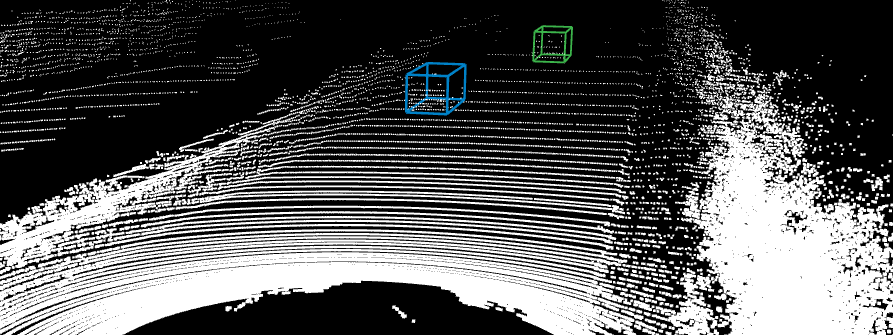
\includegraphics[width=1\linewidth]{images/supplementary/06/pc/04.png}\vspace{1pt}
	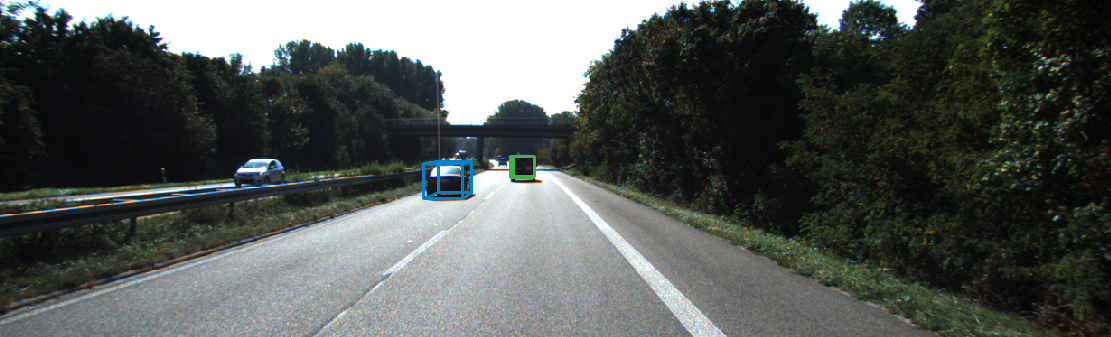
\includegraphics[width=1\linewidth]{images/supplementary/06/img/04.png}\vspace{3.55pt}
	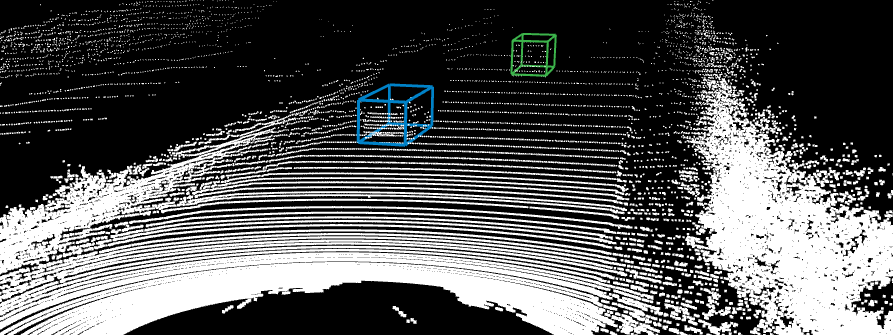
\includegraphics[width=1\linewidth]{images/supplementary/06/pc/03.png}\vspace{1pt}
	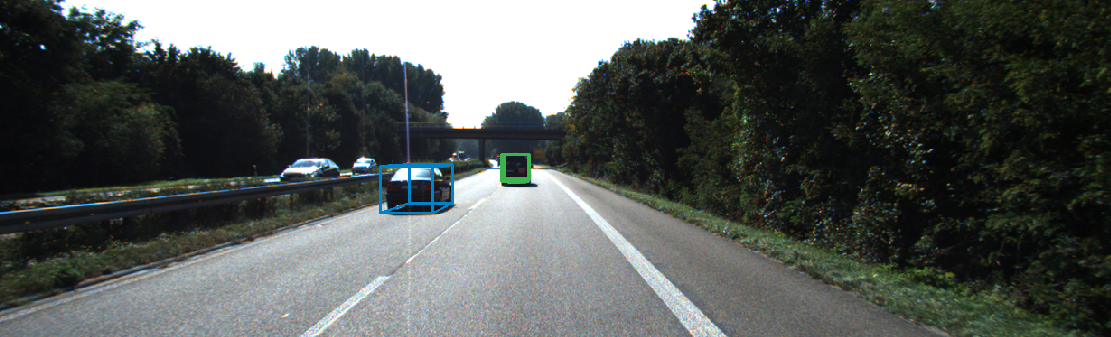
\includegraphics[width=1\linewidth]{images/supplementary/06/img/03.png}\vspace{3.55pt}
	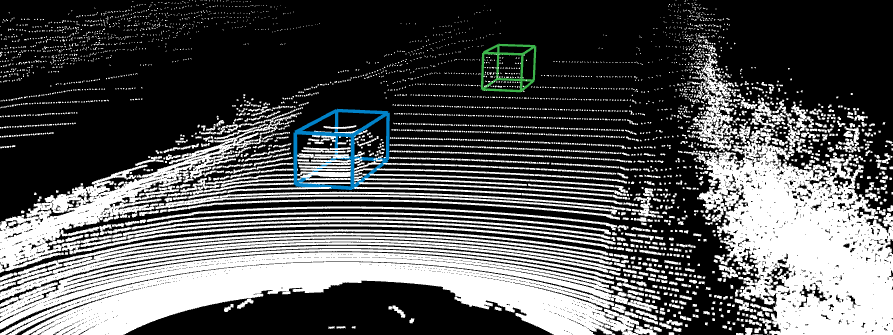
\includegraphics[width=1\linewidth]{images/supplementary/06/pc/02.png}\vspace{1pt}
	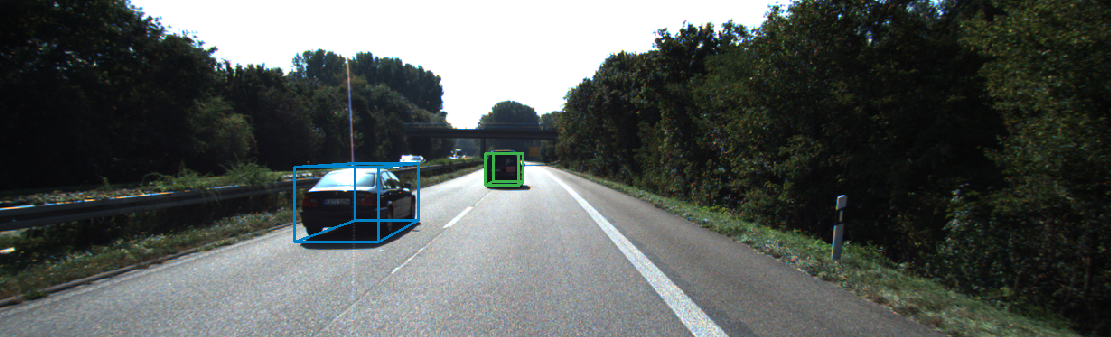
\includegraphics[width=1\linewidth]{images/supplementary/06/img/02.png}\vspace{3.55pt}
	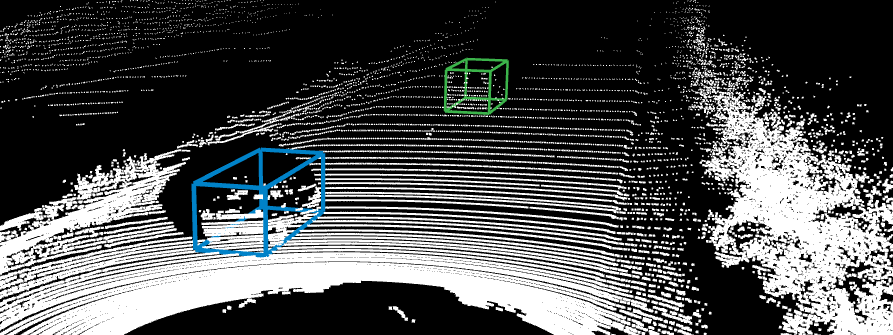
\includegraphics[width=1\linewidth]{images/supplementary/06/pc/01.png}\vspace{1pt}
	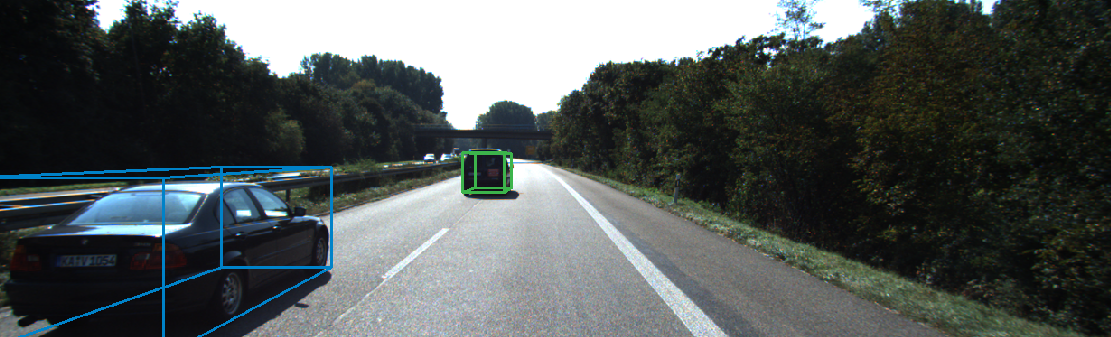
\includegraphics[width=1\linewidth]{images/supplementary/06/img/01.png}
	\end{minipage}}
	\caption{A set of trajectories of sequence 6.}
\end{figure*}

\begin{figure*}
	\centering
	\subfigure{
		\begin{minipage}[b]{0.45\linewidth}
			\begin{overpic}[scale=0.1985]{images/supplementary/10/bev/04.png}
				\put(5, 55){\color{red}{\small T = 3}}
			\end{overpic}\vspace{2pt}
			\begin{overpic}[scale=0.1985]{images/supplementary/10/bev/03.png}
				\put(5, 55){\color{red}{\small T = 2}}
			\end{overpic}\vspace{2pt}
			\begin{overpic}[scale=0.1985]{images/supplementary/10/bev/02.png}
				\put(5, 55){\color{red}{\small T = 1}}
			\end{overpic}\vspace{2pt}
			\begin{overpic}[scale=0.1985]{images/supplementary/10/bev/01.png}
				\put(5, 55){\color{red}{\small T = 0}}
			\end{overpic}
	\end{minipage}}
	\subfigure{
		\begin{minipage}[b]{0.45\linewidth}
			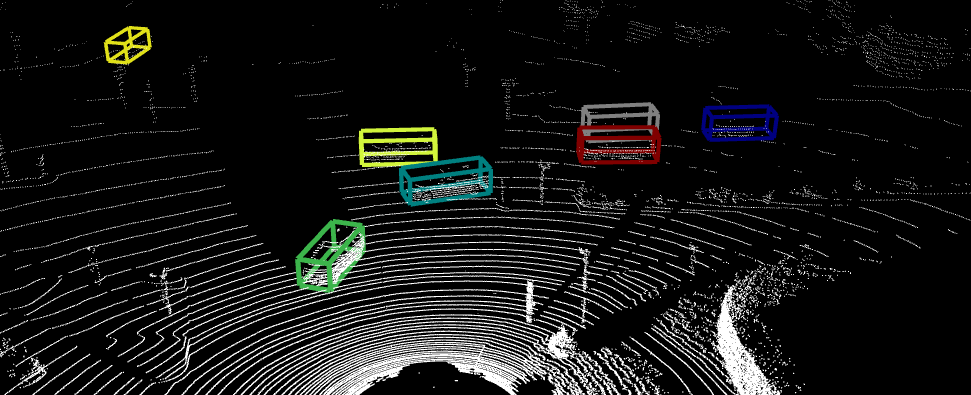
\includegraphics[width=1\linewidth]{images/supplementary/10/pc/04.png}\vspace{1pt}
			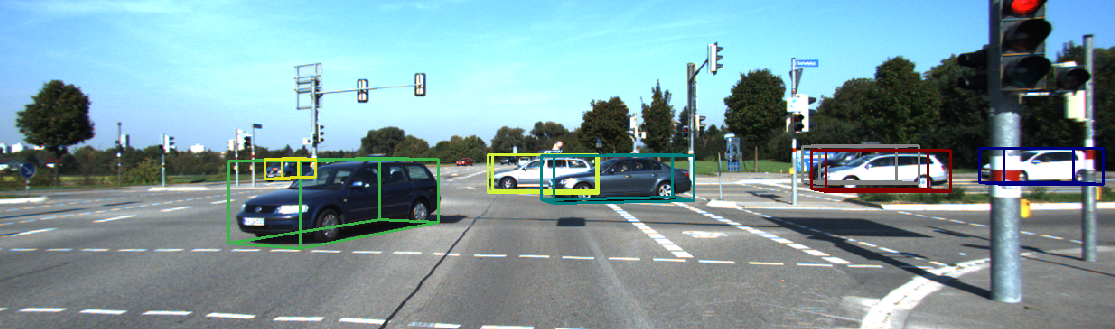
\includegraphics[width=1\linewidth]{images/supplementary/10/img/04.png}\vspace{3.55pt}
			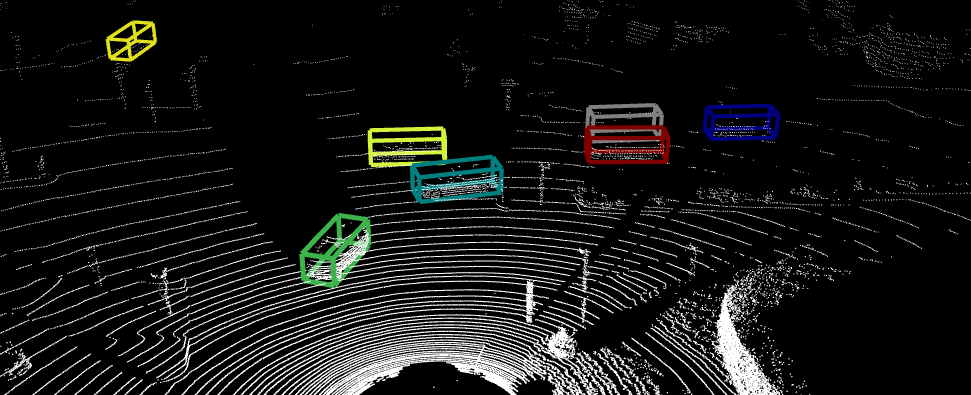
\includegraphics[width=1\linewidth]{images/supplementary/10/pc/03.png}\vspace{1pt}
			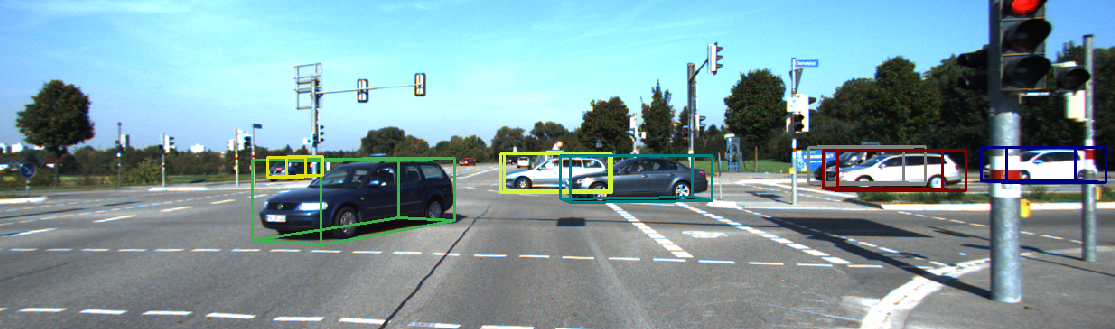
\includegraphics[width=1\linewidth]{images/supplementary/10/img/03.png}\vspace{3.55pt}
			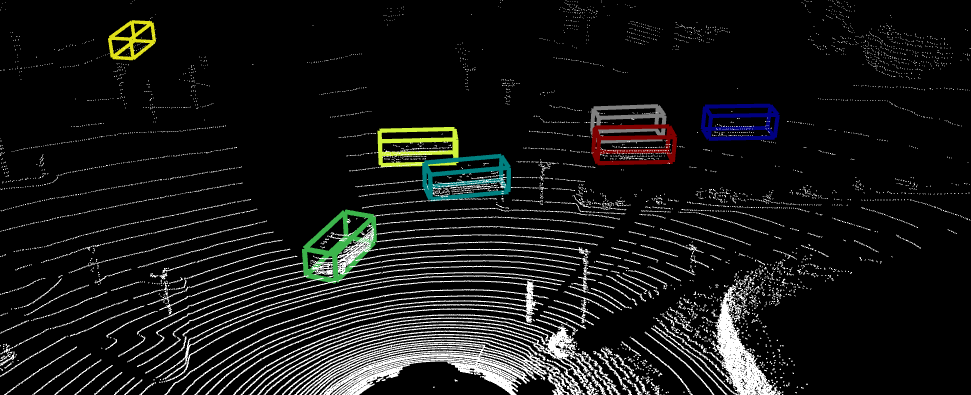
\includegraphics[width=1\linewidth]{images/supplementary/10/pc/02.png}\vspace{1pt}
			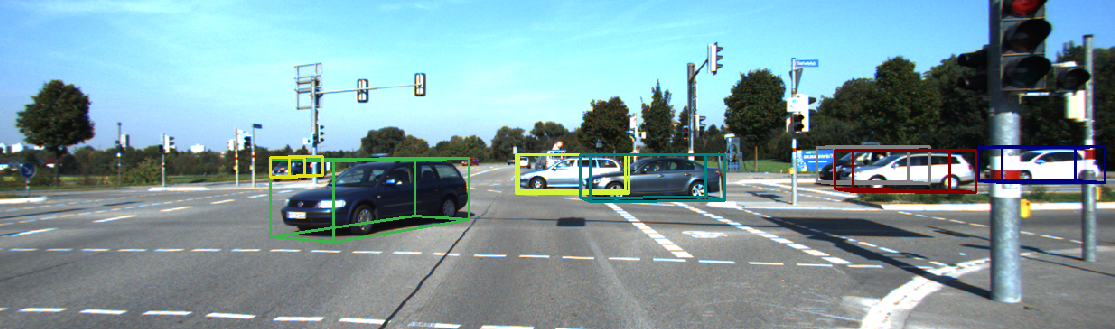
\includegraphics[width=1\linewidth]{images/supplementary/10/img/02.png}\vspace{3.55pt}
			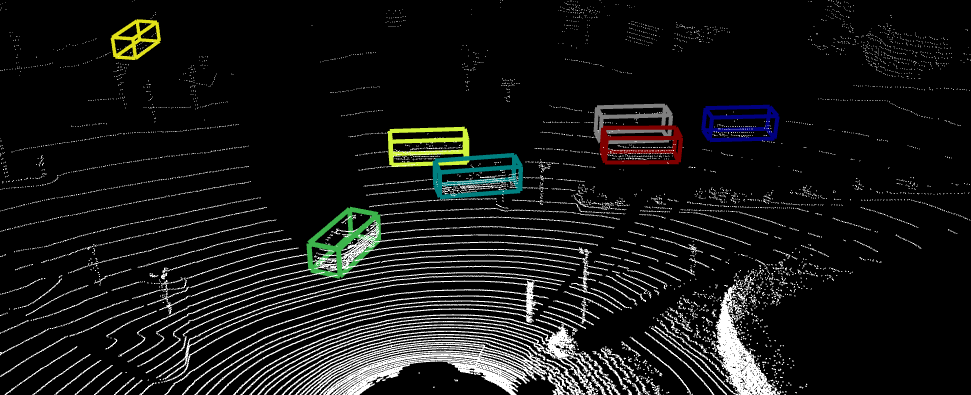
\includegraphics[width=1\linewidth]{images/supplementary/10/pc/01.png}\vspace{1pt}
			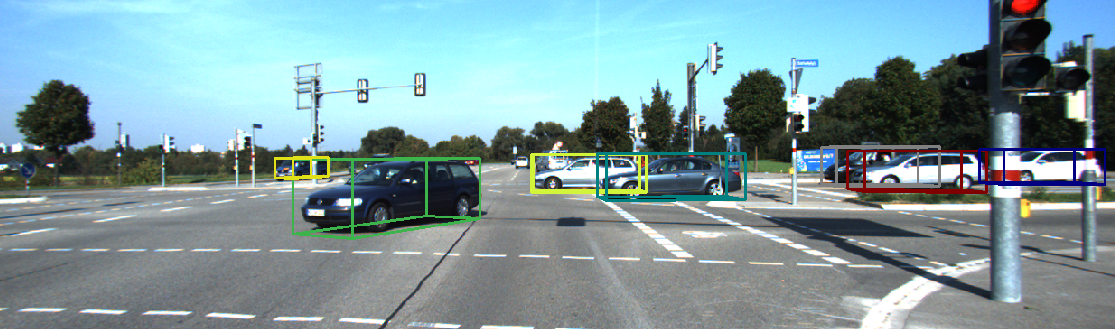
\includegraphics[width=1\linewidth]{images/supplementary/10/img/01.png}
	\end{minipage}}
	\caption{A set of trajectories of sequence 10.}
\end{figure*}


\begin{figure*}
	\centering
	\subfigure{
	\begin{minipage}[b]{0.32\linewidth}
	\begin{flushright}
		\begin{overpic}[trim={0cm, 3cm, 0cm, 0cm}, clip, scale=0.177]{images/supplementary/11/bev/04.png}
			\put(5, 88){\color{red}{\small T = 3}}
		\end{overpic}\vspace{1pt}
		\begin{overpic}[trim={0cm, 3cm, 0cm, 0cm}, clip, scale=0.177]{images/supplementary/11/bev/03.png}
			\put(5, 88){\color{red}{\small T = 2}}
		\end{overpic}\vspace{1pt}
		\begin{overpic}[trim={0cm, 3cm, 0cm, 0cm}, clip, scale=0.177]{images/supplementary/11/bev/02.png}
			\put(5, 88){\color{red}{\small T = 1}}
		\end{overpic}\vspace{1pt}
		\begin{overpic}[trim={0cm, 3cm, 0cm, 0cm}, clip, scale=0.177]{images/supplementary/11/bev/01.png}
			\put(5, 88){\color{red}{\small T = 0}}
		\end{overpic}
	\end{flushright}
	
	\end{minipage}}
	\subfigure{
	\begin{minipage}[b]{0.45\linewidth}
	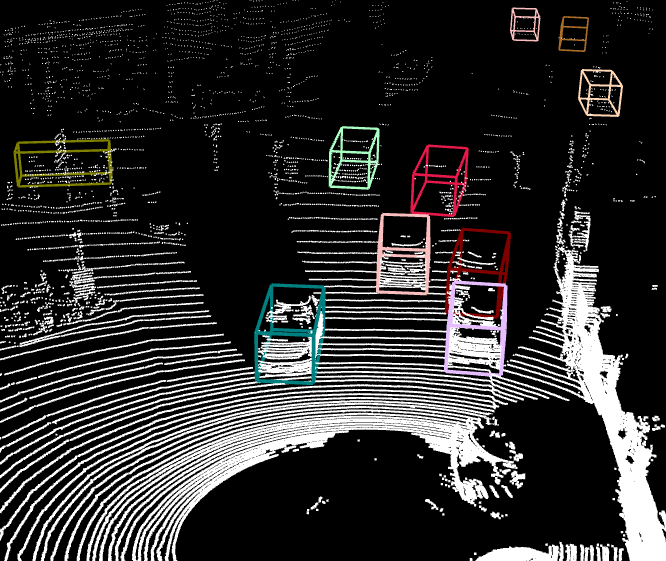
\includegraphics[trim={0cm, 5.5cm, 0cm, 0cm}, clip,width=0.85\linewidth]{images/supplementary/11/pc/04.png}\vspace{1pt}
	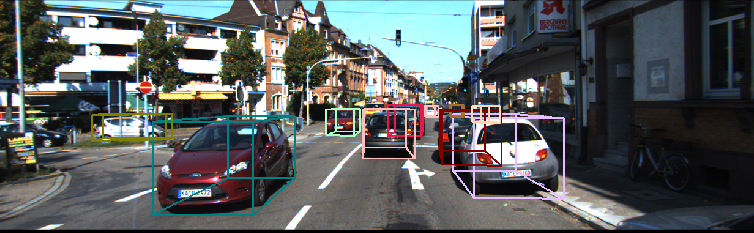
\includegraphics[width=0.85\linewidth]{images/supplementary/11/img/04.png}\vspace{1.5pt}
	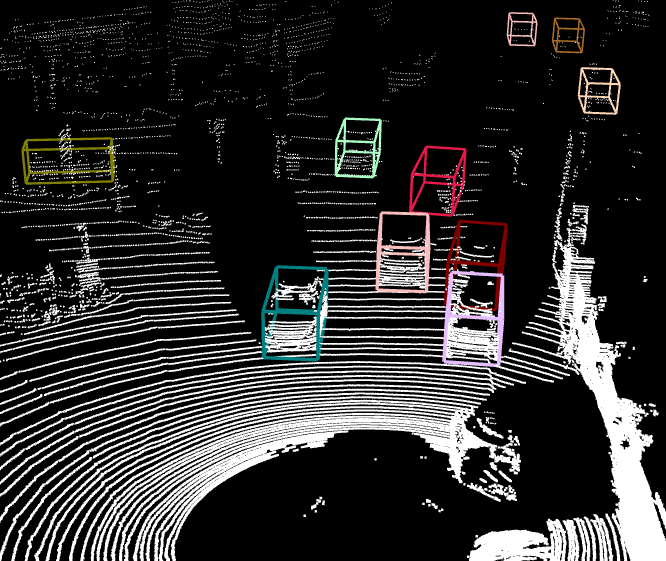
\includegraphics[trim={0cm, 5.5cm, 0cm, 0cm}, clip,width=0.85\linewidth]{images/supplementary/11/pc/03.png}\vspace{1pt}
	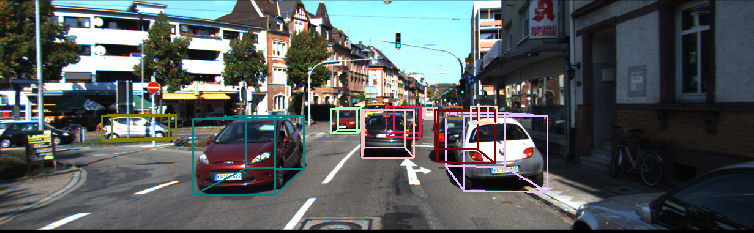
\includegraphics[width=0.85\linewidth]{images/supplementary/11/img/03.png}\vspace{1.5pt}
	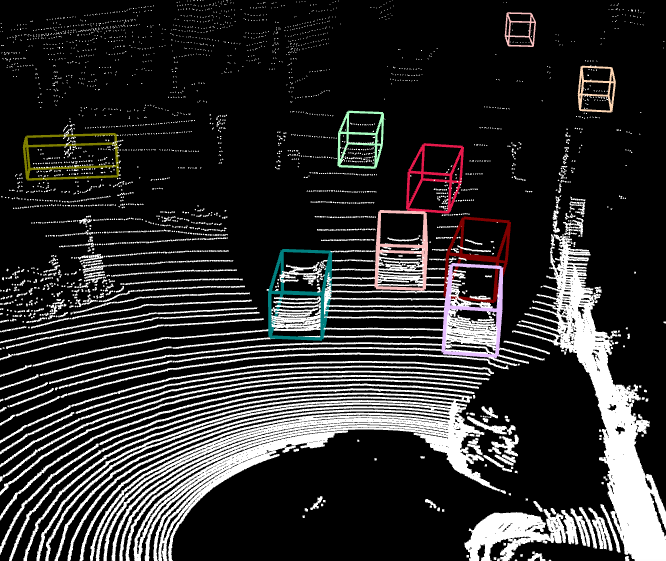
\includegraphics[trim={0cm, 5.5cm, 0cm, 0cm}, clip,width=0.85\linewidth]{images/supplementary/11/pc/02.png}\vspace{1pt}
	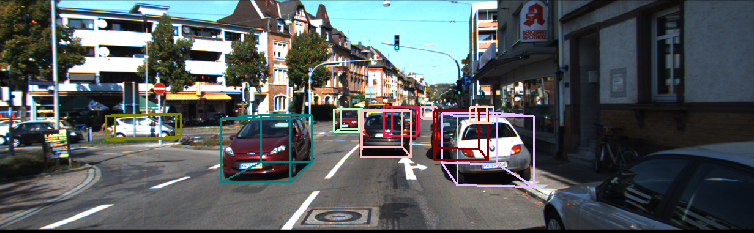
\includegraphics[width=0.85\linewidth]{images/supplementary/11/img/02.png}\vspace{1.5pt}
	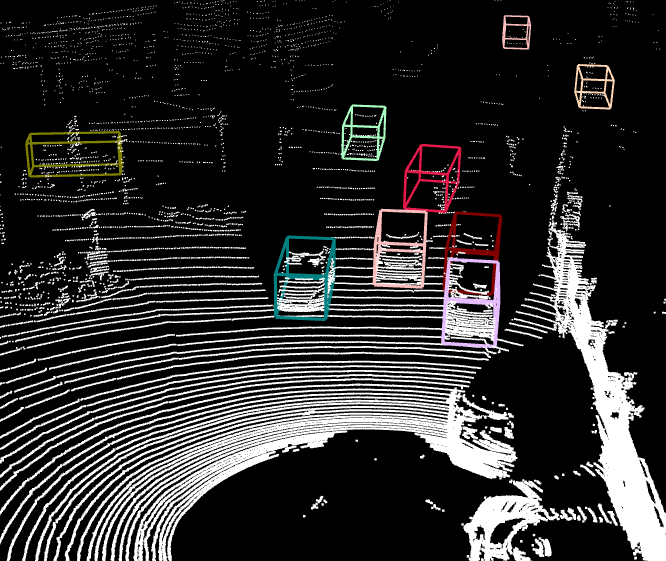
\includegraphics[trim={0cm, 5.5cm, 0cm, 0cm}, clip,width=0.85\linewidth]{images/supplementary/11/pc/01.png}\vspace{1pt}
	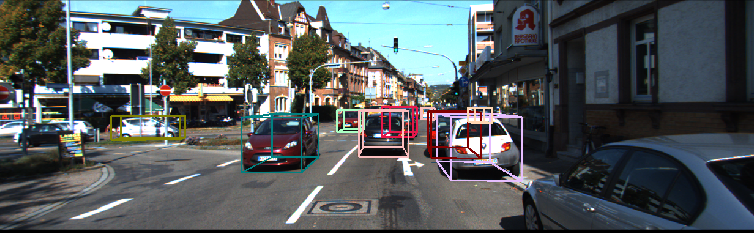
\includegraphics[width=0.85\linewidth]{images/supplementary/11/img/01.png}
	\end{minipage}}
	\caption{A set of trajectories of sequence 11.}
\end{figure*}


\begin{figure*}
	\centering
	\subfigure{
	\begin{minipage}[b]{0.4\linewidth}
	\begin{flushright}
		\begin{overpic}[scale=0.171]{images/supplementary/12/bev/04.png}
			\put(5, 87){\color{red}{\small T = 3}}
		\end{overpic}\vspace{1pt}
		\begin{overpic}[scale=0.171]{images/supplementary/12/bev/03.png}
			\put(5, 87){\color{red}{\small T = 2}}
		\end{overpic}\vspace{1pt}
		\begin{overpic}[scale=0.171]{images/supplementary/12/bev/02.png}
			\put(5, 87){\color{red}{\small T = 1}}
		\end{overpic}\vspace{1pt}
		\begin{overpic}[scale=0.171]{images/supplementary/12/bev/01.png}
			\put(5, 87){\color{red}{\small T = 0}}
		\end{overpic}
	\end{flushright}
	\end{minipage}}
	\subfigure{
	\begin{minipage}[b]{0.5\linewidth}
	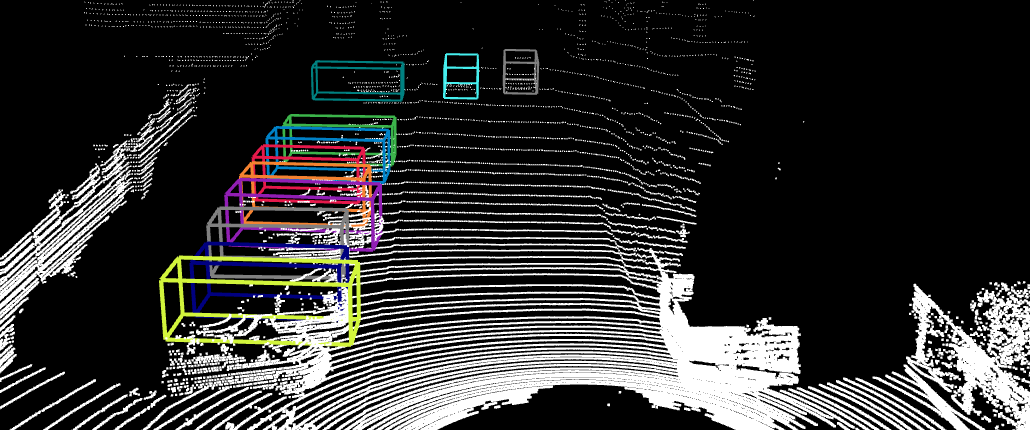
\includegraphics[width=0.95\linewidth]{images/supplementary/12/pc/04.png}\vspace{1pt}
	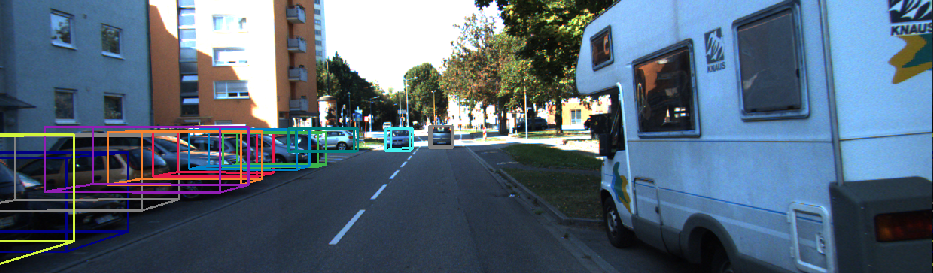
\includegraphics[width=0.95\linewidth]{images/supplementary/12/img/04.png}\vspace{1.5pt}
	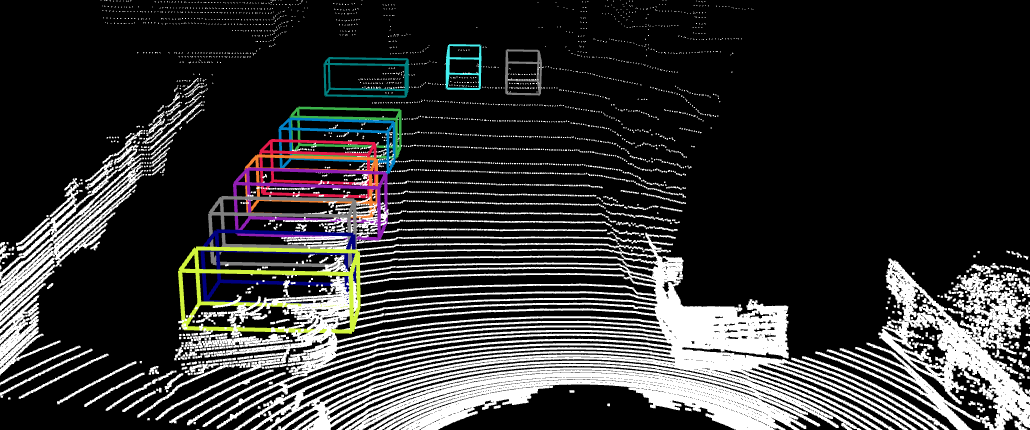
\includegraphics[width=0.95\linewidth]{images/supplementary/12/pc/03.png}\vspace{1pt}
	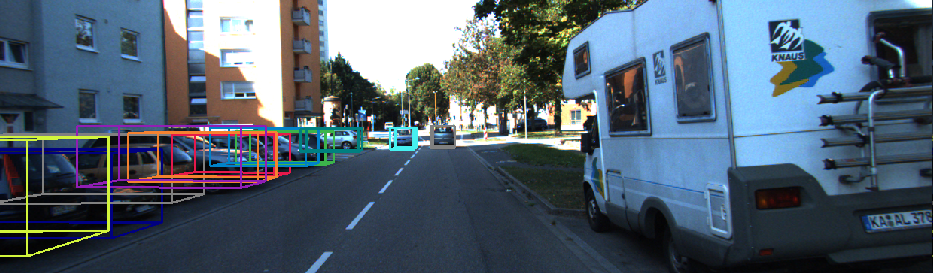
\includegraphics[width=0.95\linewidth]{images/supplementary/12/img/03.png}\vspace{1.5pt}
	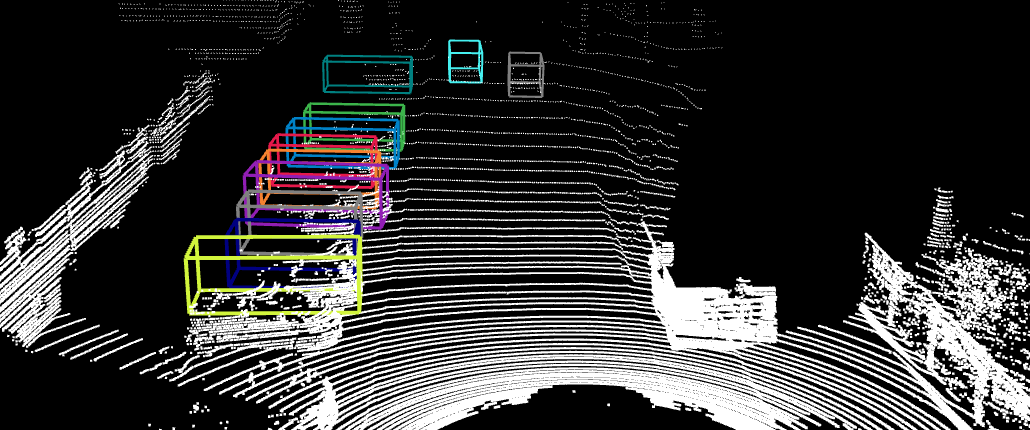
\includegraphics[width=0.95\linewidth]{images/supplementary/12/pc/02.png}\vspace{1pt}
	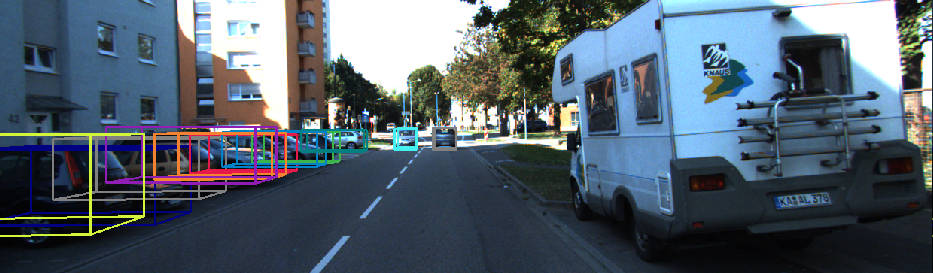
\includegraphics[width=0.95\linewidth]{images/supplementary/12/img/02.png}\vspace{1.5pt}
	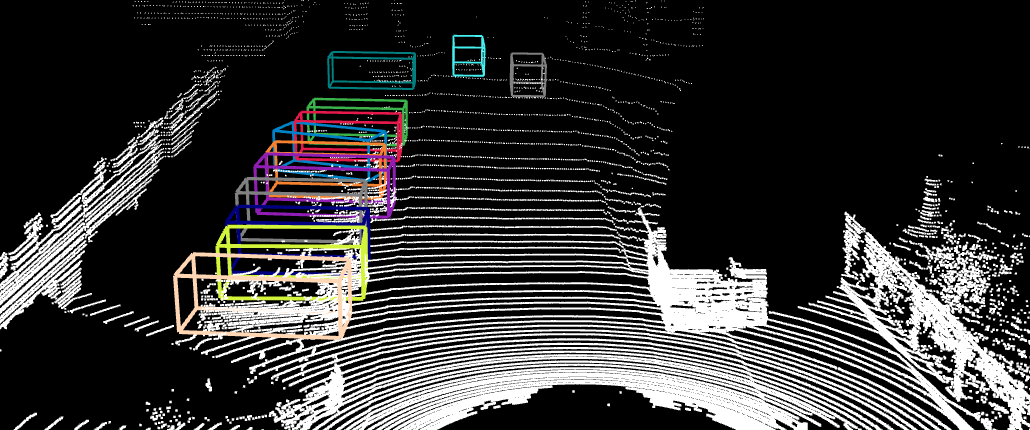
\includegraphics[width=0.95\linewidth]{images/supplementary/12/pc/01.png}\vspace{1pt}
	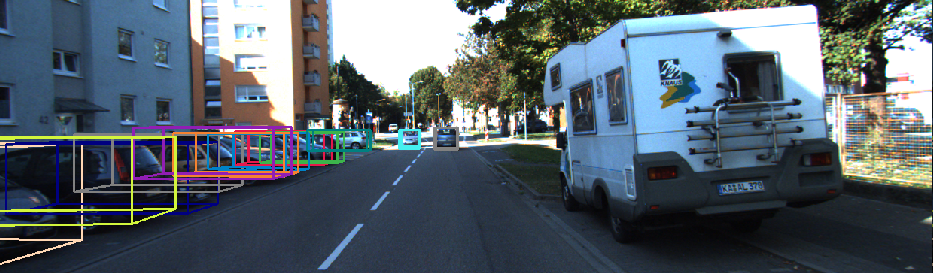
\includegraphics[width=0.95\linewidth]{images/supplementary/12/img/01.png}
	\end{minipage}}
	\caption{A set of trajectories of sequence 12.}
\end{figure*}

\end{document}